\documentclass[border=6pt]{standalone}
\usepackage{tikz}
\usetikzlibrary{arrows.meta,calc,positioning,shapes.geometric}
\begin{document}
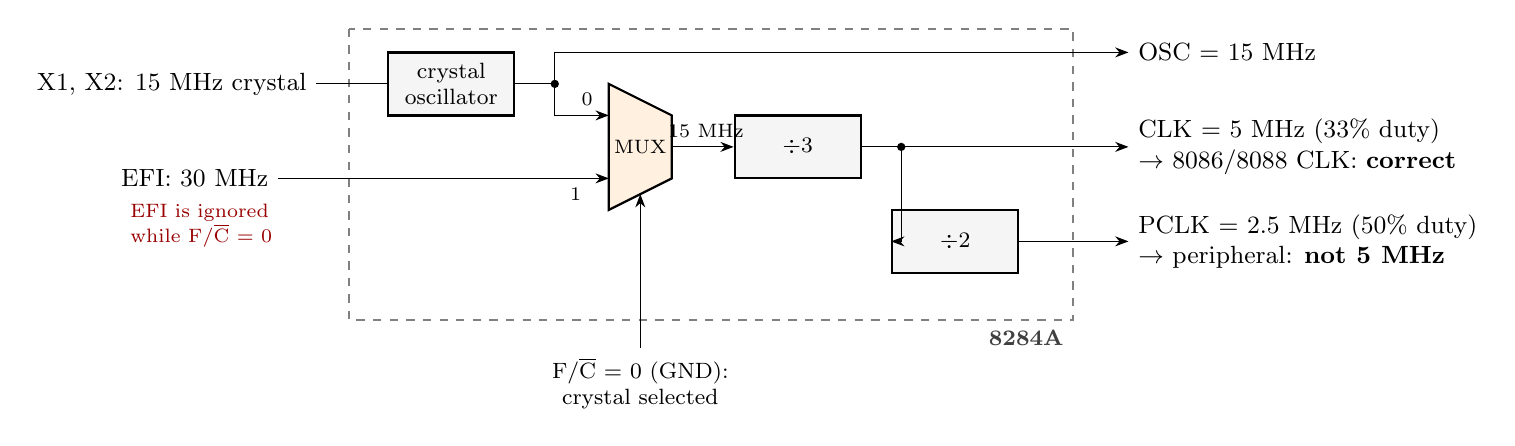
\begin{tikzpicture}[>=Stealth,font=\small,
 blk/.style={draw,thick,fill=gray!8,align=center,font=\footnotesize,minimum height=0.8cm,minimum width=1.6cm}]
\draw[thick,dashed,gray] (-0.3,1.3) rectangle (8.9,-2.4);
\node[font=\footnotesize\bfseries,gray!50!black,anchor=north east] at (8.9,-2.4) {8284A};
\node[blk] (osc) at (1.0,0.6) {crystal\\oscillator};
\draw[thick,fill=orange!12] (3.0,0.6) -- (3.8,0.2) -- (3.8,-0.6) -- (3.0,-1.0) -- cycle;
\coordinate (mux) at (3.4,-0.2);
\node[font=\scriptsize] at (3.4,-0.2) {MUX};
\node[blk] (d3) at (5.4,-0.2) {$\div 3$};
\node[blk] (d2) at (7.4,-1.4) {$\div 2$};
\draw (osc.west) -- ++(-0.9,0) node[left]{X1, X2: 15 MHz crystal};
\draw[->] (osc.east) -- ++(0.5,0) coordinate (j) |- (3.0,0.2) node[pos=0.8,above,font=\scriptsize]{0};
\draw[->] (-1.2,-0.6) node[left]{EFI: 30 MHz} -- (3.0,-0.6) node[pos=0.9,below,font=\scriptsize]{1};
\fill (j) circle (1.5pt);
\draw[->] (j) |- (9.6,1.0) node[right]{OSC = 15 MHz};
\draw[<-] (3.4,-0.8) -- (3.4,-2.75) node[below,align=center,font=\footnotesize]{F/$\overline{\mathrm{C}}$ = 0 (GND):\\crystal selected};
\draw[->] (3.8,-0.2) -- (d3.west) node[pos=0.55,above,font=\scriptsize]{15 MHz};
\draw[->] (d3.east) -- ++(0.5,0) coordinate (k) -- (9.6,-0.2) node[right,align=left]{CLK = 5 MHz (33\% duty)\\$\to$ 8086/8088 CLK: \textbf{correct}};
\fill (k) circle (1.5pt);
\draw[->] (k) |- (d2.west);
\draw[->] (d2.east) -- (9.6,-1.4) node[right,align=left]{PCLK = 2.5 MHz (50\% duty)\\$\to$ peripheral: \textbf{not 5 MHz}};
\node[font=\scriptsize,red!60!black,align=left,anchor=north west] at (-3.2,-0.8) {EFI is ignored\\while F/$\overline{\mathrm{C}}$ = 0};
\end{tikzpicture}
\end{document}
